% !TEX root = ../dissertation.tex

\chapter{Computational Geometry}

Computational geometry is defined as the systematic study of algorithms and data structures for geometric objects~\cite{berg2008}.
A specific focus is on exact algorithms that are asymptotically fast.
Computational geometry emerged from the fields of computer science in the late 1970s.
Since that time, the field has grown considerably and has found applications in a large variety of domains, suchs as computer graphics, \gls{gis}, robotics, \gls{CAD}, computer vision, and others.

The general approach to solving computational geometric problem is based on two key components.
The first is a deep understanding of the geometric properties of the problem and the second is the proper application of efficient algorithms and/or data structures.
In this chapter, we use several algorithms and approaches from computational geometry to simulate a spacecraft mounted \gls{lidar} sensor around an asteroid.
The first task is to simulate the measurement from the \gls{lidar} of the surface of the asteroid.
This will utilize the well known method of \gls{raycasting} to find the intersection of a mesurement ray with the surface.
Given the surface intersection, these measurements will be incrementally incoprorated into the asteroid shape model while maintaining the required topological constraints.

\section{Mathematical Background}

% TODO Come up with some consistent notation
\begin{itemize}
    \item Talk about polygon/polyhedron backgroudn
    \item Define euler's equation
    \item Talk about all the background in convex, sets, connectivity, topology etc.
    \item Come up with a consistent notation for the entire thing
\end{itemize}

The \gls{polyhedron} potential model is the standard approach for missions around asteroids~\cite{werner1996,werner1994}.
As a result, an understanding of the properties of \glspl{polyhedron} and the methods to construct them are critical.
The construction and update of the asteroid shape model must produce a valid three-dimensional model.
For example, the geometric model must not contain any dangling edges or surfaces~\cite{mortenson1997}.
A consideration of the topology of the model is crucial, and features such as homogenity and connectivity are important properties to consider.

A \gls{polyhedron} is an arrangement of \glspl{polygon} such that two and only two \glspl{polygon} meet at an edge~\cite{mortenson1997}.
Furthermore, it is possible to travese the surface of the \gls{polyhedron} by crossing it's edges to eventually cross each face in a continuous path.

\subsection{Polyhedra}

A polyhedron is a generalization of a two-dimensional polygon to three-dimensions.
It is the region of space with a boundary defined by a surface of a finite number of polygonal faces.
The surface of the polyhedron is composed of three types of primitive objects: zero-dimensional points called vertices, one-dimensional segments called edges, and two-dimensional polygons called faces or facets.
Furthemore, without any loss of generality we assume each face is a convex polygon since any nonconvex face can be divided into smaller convex faces.
A valid polyhedron in the context of asteroid shape models must satisfy several constraints.
These constraints define the relationship between each of the types of primitives which make up the polyhedron surface.
The primitives must intersect ``properly'', the local and global topology must be ``proper''.
For asteroid shape model we further assume that each face is a triangular polygon. 
Again, this does not limit generality as any polygon can be divided into a series of planar triangles.

The intersection of each face must be one of the following:
\begin{itemize}
    \item the faces are disjoint and do not intersect, or
    \item the faces meet at a single vertex, or
    \item the faces share two vertices and a common edge.
\end{itemize}
This constraint automatically ensures that all edgeds and vertices intersect properly.
Improper intersection would penetrating faces and faces that intersect improperly. 
Such as an edge not extending across an entire face.

The second constraint is related to the local topology around each point of the polyhedron.
In order to be locally proper, the neighborhood about any point on the surface of the polyhedron should be homeomorphic to a two-dimensional disk.
A neighborhood about any point on the surface is defined as an arbitrarily small subset or region of the surface which surrounds the point.
Every point on the surface should have a neighborhood which is topologically equivalent to a two dimensional disk.
The notion of equivalency is mathematically captured using the property of \gls{homeomorphism}.
A homemorphism between two regions is a continous stretching or bending, without tearing or cutting, from one shape to another.
This constraint will exlude objects that are not proper polyhedrons, for example those shown in~\cref{fig:improper_polyhedrons}.
\begin{figure}[h]
    \centering
    \subcaptionbox{Point lies on two surfaces\label{fig:two_surfaces}}{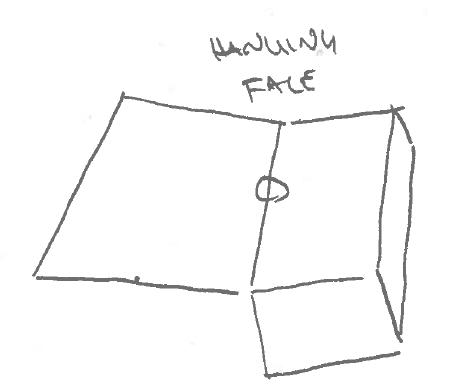
\includegraphics[width=0.33\textwidth]{figures/computational_geometry/hanging_face.png}}~
    \subcaptionbox{The neighborhood around this point is not homemorphic to a disk\label{fig:knotted_polyhedron}}{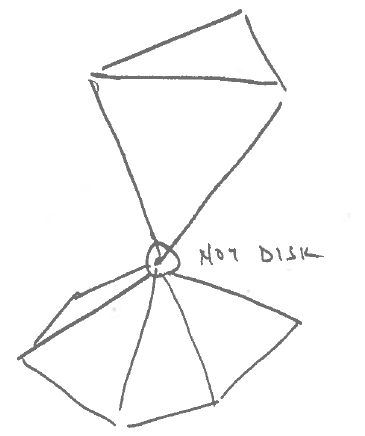
\includegraphics[width=0.33\textwidth]{figures/computational_geometry/pinched.png}}~
    \subcaptionbox{The surface is not closed\label{fig:open_polyhedron}}{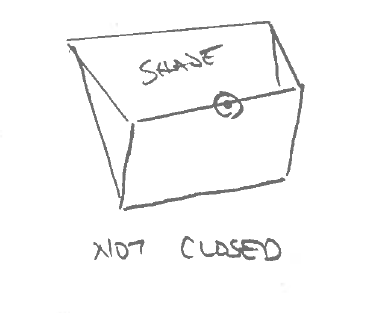
\includegraphics[width=0.33\textwidth]{figures/computational_geometry/open.png}}
    \caption{Three example objects which are not polyhedra. For each example, the neighborhood about each point is not homeomorphic to an open disk.~\label{fig:improper_polyhedrons}}
\end{figure}
In a neighborhood about any point on the surface of the polyhedron should be equivalent to that of a two-dimensional disk.
A surface where this true for all points is called a \textit{two-manifold}, of a which the surface of a polyhedron is a subset.

The final constraint is related to the global structure of the surface in contrast to the local neighborhood of a point.
The surface must be connected, closed, and bounded.

\begin{itemize}
    \item Talk about 2-manifold and homeomorphism to a disk
    \item Define neighborhood of each point (open adn closed balls)
\end{itemize}

Global topology
\begin{itemize}
    \item Connected closed and bounded
    \item talk about closed holes (torus) and the genus of a polyhedron
\end{itemize}

Platonic solids
\begin{itemize}
    \item Talk about platonic solids and Euler's equation
\end{itemize}

\subsection{Area of a Polyhedron}
There is a simple method for determining the volume of an polyhedron.
Here we present a straightforward derivation of the formula beginning with the area of a planar polygon and extending to that of a polyhedron.
The full derivation can be found in~\citeauthor{newson1899}.
Discuss the computation of the area of a polyhedron~\cite{newson1899}.
\section{Incremental Mesh update}

This section we outline our algorithm to incrementally update a mesh. 
Some assumptions:

\begin{itemize}
    \item We first assume that the initial shape model of the asteroid is valid, though not necessarily accurate.
        This means that the mesh is a closed, regular triangular polyhedron.
    \item We assume that there is a sufficient number of vertices in the initial mesh. 
        Therefore during the surface reconstruction phase, the total number of vertices will not vary greatly.
\end{itemize}

The algorithm to insert a point into a given mesh is:

\begin{enumerate}
    \item Determine the distance from the candidate vertex to the mesh.
    \item Identify the closest ``primitive'', i.e. the closest edge, face, or vertex to the candidate point
    \item Incorporate the candidate point into the mesh
\end{enumerate}

There are three possibilities for the closest primitive to the candidate point. 
Based on the distance, there is a different procedure to incorporate the point.

\subsection{Distance to the mesh}

In order to incorporate a given measurement into the mesh, first the distance to the mesh must be determined.
Specifically, the closest point of the mesh is required to determine the manner in which to to update the mesh.
This section presents the approach used to determine the distance from a candidate vertex to the exisisting mesh. 
The subsequent sections demonstrate how to use this information to update the mesh, while maintaining the topology of the polyhedron.

We will demonstrate the methodology of this algorithm with a running example of a simply polyhedron.
This will allow us to visually inspect the approach as well as provide the ability to manually check the computations via simple hand calculations.
Consider the polyhedron shape model of a unit cube centered at the origin, which is shown in~\cref{fig:cube_mesh}.
\begin{figure}
    \centering
    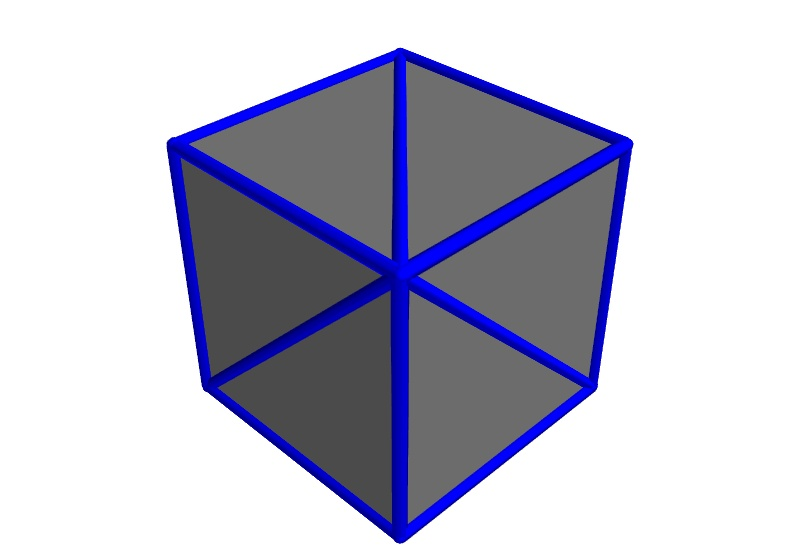
\includegraphics[width=\textwidth]{figures/computational_geometry/cube_mesh.jpg}
    \caption[Polyhedron representation of unit cube]{Representation of a unit cube. The edges are defined in red, the vertices in blue, and the faces in gray.~\label{fig:cube_mesh}}
\end{figure}
The polyhedron is defined entirely by the locations of the vertices and the connectivity between vertices to define the triangular faces.
Each vertex of the cube, \( \vb{v}_i \in \R^3\), is stored in a large vertex array \( \vb{V} \in \R^{v \times 3} \), as shown in~\cref{eq:cube_vertex_array}.
The vertices for all polyhedron shape models are typically defined in a body fixed reference system centered at the origin of the shape and aligned with the priniciple axes of the body.
\begin{align}~\label{eq:cube_vertex_array}
    \vb{V} = \begin{bmatrix}
        \begin{array}{ccc}
        -0.5 & -0.5 & -0.5 \\
        -0.5 & -0.5 & 0.5  \\
        -0.5 & 0.5  & -0.5 \\
        -0.5 & 0.5  & 0.5  \\
        0.5  & -0.5 & -0.5 \\
        0.5  & -0.5 & 0.5  \\
        0.5  & 0.5  & -0.5 \\
        0.5  & 0.5  & 0.5
    \end{array}
   \end{bmatrix}.
\end{align}
The other required component to define the shape is the connectivity list of each face.
Each triangular face, or facet, of the surface is defined as a triangular face consisting of the three vertices which define the polygon.
Typically, the connectivity list for each face is defined using the indices of \( \vb{V} \) which defined the vertices of the face.
For the unit cube, each face, \( \vb{f}_i \in \R^3\) is stored in a large face array \( \vb{F} \in \R^{f \times 3}\), as shown in~\cref{eq:cube_face_array}.
\begin{align}\label{eq:cube_face_array}
    \vb{F} = 
    \begin{bmatrix}
        \begin{array}{ccc}
            0 & 6 & 4 \\
            0 & 2 & 6 \\
            0 & 3 & 2 \\
            0 & 1 & 3 \\
            2 & 7 & 6 \\
            2 & 3 & 7 \\
            4 & 6 & 7 \\
            4 & 7 & 5 \\
            0 & 4 & 5 \\
            0 & 5 & 1 \\
            1 & 5 & 7 \\
            1 & 7 & 3
        \end{array}
    \end{bmatrix}.
\end{align}
For example, using~\cref{eq:cube_face_array} we can see that the first face, \( \vb{f}_0 = \begin{bmatrix}\begin{array}{ccc} 0 & 6 & 4 \end{array}\end{bmatrix}\), is defined by the following vertices
\begin{align*}
    \vb{v}_0 &= \begin{bmatrix} \begin{array}{ccc} -0.5 & -0.5 & -0.5\end{array}\end{bmatrix},\\
    \vb{v}_6 &= \begin{bmatrix}\begin{array}{ccc} 0.5 & 0.5 & -0.5 \end{array}\end{bmatrix}, \\
    \vb{v}_4 &= \begin{bmatrix}\begin{array}{ccc}  0.5  & -0.5  & -0.5\end{array}\end{bmatrix}.
\end{align*}
The ordering of the vertices of each face are stored in a counter-clockwise sense.
As a result, the explicit definition of the face normal is unnessary as the standard will automatically ensure that all face normals are outward pointing.
This type of representation is common in the computational geometry field is typically referred to as the Wavefront OBJ format.
Furthermore, this format is the common standard for the definition of asteroid shapes by NASA \gls{pds}~\cite{gaskell2008b,gaskell2008a}
\subsection{Distance to Vertices}

\begin{enumerate}
    \item Find \( L_2\) norm from \( p \) to each vertex \( v \in V\)
    \item \( V \) -- Find minimum distance, and the index of the associated vertex
    \item \( F \) -- Determine all faces that contain this vertex, 
    \item \( E \) -- Find all edges with this vertex
    \item \( N \) -- Determine normals associated with connected faces \( F \)
    \item \( \pm D\) -- determine signed distance, \( N \cdot \parenth{p - P}\)
\end{enumerate}

\subsection{Distance to Edges}
The key difference is that we want to identify the closest edge and output the minimum distance location on that edge.
Furthermore, we need to ensure that this minimum distance point actually is contained by the edge.

Given : \( x_1, x_2 \in \R^3\) defining the vertices of a given edge. 

\begin{enumerate}
    \item Parametric form of edge \( v = x_1 + \parenth{x_2 - x_1} t\) with \( t \in \bracket{0, 1} \)
    \item Distance from \( p \) to \( v(t) \)
        \begin{align}
            d^2 &= \norm{v(t) - p}^2 
        \end{align}
    \item Minimum distance is found by finding \( t\) which minimizes \( d^2 \)
        \begin{align}
            t = - \frac{\parenth{x_1 - p} \cdot \parenth{x_2 - x_1}}{\norm{x_2 - x_1}^2}
        \end{align}
        Make sure that the value lies in \( t \in \bracket{0, 1}\) or else the perpindicular minimum distance lies outside of the edge.
    \item Then we can find \( d \) by using the solved value of \( t \)
        \begin{align}
            d = \frac{\parenth{x_1 - x_0} \cdot \parenth{x_2 - x_1}}{\norm{x_2 - x_1}}
        \end{align}
    \item \(P\) -- Location of closest point on surface
    \item \( E\) -- identify the minimum edge
    \item \( V\) -- Identify vertices that define this edge
    \item \( F\) -- Identify the faces which hold this edge
    \item \( \pm D\) -- Signed distance to \( p\) similar to above
\end{enumerate}

\subsection{Distance to Faces}
This is again more complicated as we now want to find the minimum distance to a plane.
In addition, we'd like to output this point and ensure it lies within the surface.

Given : Plane defined by \( v_1, v_2, v_3 \in \R^3\)
\begin{enumerate}
    \item Find normal projection of \( p \) onto the plane
    \item Define parametric line from \( p \) in direction of \( - \hat n \)
        \begin{align}
            p_0 = p - t \hat n
        \end{align}
    \item Find parameter which defines distance to plane and the location of intersection point
        \begin{align}
            t = \hat n \cdot p - \hat n \cdot v_1
        \end{align}
    \item Need to determine the barycentric coordinates of the intersection point \( p_0\) and see if it is inside or outside of the plane
        \begin{align}
            \alpha v_1 + \beta v_2 + \gamma v_3 = p_0
        \end{align}
\end{enumerate}

\subsubsection{Barycentric Coordinates}

Given : \( p_0 in \R^3\) in the plane defined by \( v_1, v_2, v_3 \in R^3\)

Find : Location of \( p_0 \) in the triangle

\begin{enumerate}
    \item Parametric equation of a plane
        \begin{align}
            \pi(s, t) = v_1 + s \parenth{v_2 - v_1} + t \parenth{v_3 - v_1}
        \end{align}
    \item \( p_0 \) lies on the plane so we can define the following
        \begin{align}
            p_0 &= v_1 + s \parenth{v_2 - v_1} + t \parenth{v_3 - v_1} \\
            c &= s a + t b
        \end{align}
        where we define the following
        \begin{align*}
            a = v_2 - v_1 \quad b= v_3- v_1 \quad c = p - v_1 \quad n = a \times b
        \end{align*}
    \item Define perpindicular vectors in the plane
        \begin{align}
            a_p = n \times a \quad b_p = n \times b
        \end{align}
    \item Solve for \( s, t\)
        \begin{align}
            s = \frac{c \cdot b_p}{a \cdot b_p} \quad t = \frac{c \cdot a_p}{b \cdot a_p}
        \end{align}
    \item Use triple product rule to simplify
        \begin{align}
            s &= \frac{\parenth{a \cdot b}\parenth{c \cdot b}-\parenth{b \cdot b} \parenth{c \cdot a}}{\parenth{a \cdot b}^2 - \parenth{b \cdot b} \parenth{ a \cdot a}} \\
            t &=  \frac{\parenth{a \cdot a}\parenth{c \cdot b}-\parenth{b \cdot a} \parenth{c \cdot a}}{\parenth{a \cdot a}^2 - \parenth{b \cdot b} \parenth{ b \cdot a}} \\
        \end{align} 
    \item Use parametric plane equation to find barycentric coordinates \( \alpha, \beta, \gamma\)
        \begin{align}
            \alpha = 1 - s -t \quad \beta = s \quad \gamma = t \quad \alpha + \beta + \gamma = 1
        \end{align}
    \item Output minimum distance \( D\), minimum location \( P \), vertices \( V \), edges \( E\), and faces \( F \)
\end{enumerate}
If the candidate point is closest to a vertex, then you can simply redefine the vertex to be the candidate point.

\section{Incremental Radius modification}
 
Here we present a simple algorithm to incrementally update a polygonal mesh with new data points.
In addition, we then demonstrate it's use with two numerical examples.
We begin by assuming we have an initial model of the asteroid in the form of a triangular mesh.
Frequently, this initial model will be a triaxial ellipsoid that serves as an initial approximation of the true asteroid shape.
The polygonal model is given in the form of vertices, \( \vb{V} \in \R^{v \times 3}\), and faces, \( \vb{F} in \R^{f \times 3} \).
The first step is to convert the cartesian coordinates into a spherical coordinate representation. 
Each vertex, \( \vb{v}_i \in \vb{V} \), can be converted to the spherical coordinates, \( r, \theta, \phi \) through the following transformation
\begin{figure}[htbp]
    \centering
    \includegraphics[width=\textwidth]{example-image-golden}
    \caption{Spherical Coordinate Transformation~\label{fig:spherical_coordinate_transformation}}
\end{figure}
\begin{align}
    r_i &= \norm{\vb{v}_i}, \\ 
    \theta_i &= \arctan{\frac{z}{r_i}}, \\
    \phi_i &= \arctan{\frac{y}{r_i}}.
\end{align}

The next step is to define a region around each candidate point that serves as the maximum area of modification. 
An infinitesimal surface area element, \( d A \), is shown in~\cref{fig:spherical_coordinate_transformation}.
Given the spherical coordinates this area is defined as
\begin{align}
    d A = r^2 \cos \theta d \phi d \theta .
\end{align}
Given a desired surface area, \( d A \), the region of interest in the \( \theta, \phi \) directions can be computed as
\begin{align}
    k d \theta ^2 = \frac{d A}{r^2 \cos \theta}, 
\end{align}
where we define \( k = \frac{ \theta}{\phi} \) as the ratio between the latitude and longitude.

The geodesic distance on a sphere can be computed given two points, \( \theta_1, \phi_1\) and \( \theta_2, \phi_2\).
From spherical geometry, the central angle is given as
\begin{align}
    \Delta \sigma = \arctan \frac{\sqrt{\parenth{\cos \theta_2 \sin \Delta \phi}^2 + \parenth{\cos \theta_1 \sin \theta_2 - \sin \theta_1 \cos \theta_2 \cos \Delta \phi}^2 }}
    {\sin \theta_1 \sin \theta_2 + \cos \theta_1 \cos \theta_2 \cos \Delta \phi} , 
\end{align}
where \( \Delta \phi = \phi_2 - \phi_1 \).
The geodesic distance is then given as a scaled value of the central angle, \( d = r \Delta \sigma\).

The vertices that lie within the region of interest
\begin{align*}
    \abs{\theta_i} &< \Delta \theta_i,  \\
    \abs{\phi_i} &< \Delta \phi_i .
\end{align*}
are modified according to the following function
\begin{align}
    r_i = r_s \parenth{r_m - r_i} + r_i
\end{align}
where the scale factor \( r_s\) is computed according to the half normal distribution
\begin{align}
    r_s = \frac{\sqrt{2}}{\sigma_s \sqrt{\pi}} \exp \parenth{ - \frac{\Delta \sigma^2}{2 \sigma_s^2} } ,
\end{align}
where \( \sigma_s > 0 \) is a scale factor to shape the radius scale curve.
\begin{figure}
    \centering
    \includegraphics[width=\textwidth]{example-image-golden}
    \caption{Radius scale factor plot~\label{fig:radius_scale_factor}}
\end{figure}

\subsection{Variations of scale factor parameters}


\subsection{Incremental mesh update}

Now that we have an effective algorithm to find the distance between a candidate point and the primitives of the surface mesh, we can investigate a method to efficiently incorporate the new candidate point.

The algorithm is composed of the following

\begin{itemize}
    \item Find the angle between the candidate point and all the vertices
    \item Determine vertices that  lie within and angular constraint
    \item Find the perpindicular projection of the candidate point on all of these vertices
    \item Find the change in radius for these vertices. 
    \item The minimum radius is the vertes that will be changed.
    \item If no vertices lie inside the angle constraint then either use the face or edge vertex addition.
\end{itemize}
